%------------------------------------------%
% Cannabis Data Science #58
% Date: 3/23/2022
%------------------------------------------%
\documentclass[xcolor={dvipsnames}]{beamer}
\hypersetup{pdfpagemode = FullScreen}
\mode<presentation>{
  \usetheme{Boadilla}
  \usecolortheme{orchid}
  \usefonttheme{default}
  \setbeamertemplate{navigation symbols}{}
  \setbeamertemplate{caption}[numbered]
}
\setbeamersize{
  text margin left = 0.5in,
  text margin right = 0.5in
}

%------------------------------------------%
% Title
%------------------------------------------%
\title[\textbf{Cannabis Data Science \#58}]{}
\author{Cannabis Data Science}
\institute[]{\Large Cannabis Data Science \#58}
\date{March \nth{23}, 2022}

%------------------------------------------%
% Packages
%------------------------------------------%
\usepackage[english]{babel}
\usepackage[utf8x]{inputenc}
\usepackage{tikz} % For styling.
\usepackage{xparse}

%------------------------------------------%
% Colors
%------------------------------------------%
\definecolor{Green}{RGB}{34, 153, 84}
\definecolor{LightGreen}{RGB}{218, 247, 166}
\definecolor{DarkGreen}{RGB}{2, 48, 32}
\definecolor{Orange}{RGB}{255, 87, 51}
\definecolor{DarkOrange}{RGB}{199, 0, 57}
\definecolor{Yellow}{RGB}{255, 195, 0}

%------------------------------------------%
% Theme
%------------------------------------------%
\setbeamercolor*{palette primary}{bg=LightGreen, fg=DarkGreen}
\setbeamercolor*{palette secondary}{bg=LightGreen, fg=DarkGreen}
\setbeamercolor*{palette tertiary}{bg=LightGreen, fg=DarkGreen}

%------------------------------------------%
% Packages
%------------------------------------------%
\usepackage{amsmath}
\renewcommand*\footnoterule{} % No separating line on footnote.
\usepackage{mathtools} % For annotating equations.
\usepackage{hhline} % for double bars.
\usepackage[super]{nth} % For formatting 1st, 2nd, 3rd, etc.
\usepackage{graphicx, caption, subcaption}
\usepackage{setspace}

%------------------------------------------%
% Commands
%------------------------------------------%

% Top space.
\newcommand\T{\rule{0pt}{2.5ex}}

% Bottom space.
\newcommand\B{\rule[-1.25ex]{0pt}{0pt}}

% Blocks.
\newenvironment<>{Block}[2][.9\textwidth]
  {\setlength{\textwidth}{#1}
  \begin{actionenv}#3
    \def\insertblocktitle{#2}\par
    \usebeamertemplate{block begin}}
  {\par\usebeamertemplate{block end}
  \end{actionenv}}

% Balls.
\defbeamertemplate{enumerate item}{largeball}
{\begin{pgfpicture}{-1ex}{-0.65ex}{1.5ex}{1.5ex}
\usebeamercolor[fg]{item projected}
{\pgftransformscale{2.5}\pgftext{\Large\pgfuseshading{bigsphere}}}
{\pgftransformshift{\pgfpoint{0pt}{0.5pt}}
\pgftext{\usebeamerfont*{item projected}\small\insertenumlabel}}
\end{pgfpicture}}

% Fancy arrows.
\NewDocumentCommand\UpArrow{O{2.0ex} O{black}}{%
   \mathrel{\tikz[baseline] \draw [->, line width=0.5pt, #2] (0,0) -- ++(0,#1);}} % Fancy up-arrow.
\NewDocumentCommand\DownArrow{O{2.0ex} O{black}}{%
   \mathrel{\tikz[baseline] \draw [<-, line width=0.5pt, #2] (0,0) -- ++(0,#1);}} % Fancy down-arrow.

% Equations with numbers on the left.
\makeatletter
\newcommand{\LeftEqNo}{\let\veqno\@@leqno}
\makeatother

%------------------------------------------%
% Presentation
%------------------------------------------%
\begin{document}

% Title page.
\begin{frame}{}
  
\includegraphics[scale=0.33]{images/logo.pdf}
  \vspace*{-2\baselineskip}
  \titlepage

  % TODO: Add flare to title page?
  % Background
%\tikz[remember picture, overlay]
%\node[opacity=1.0, inner sep=0pt] at (current page.center){
%  
\includegraphics[width=\paperwidth, height=\paperheight]{images/cover.pdf}
%};  
  
\end{frame}

%------------------------------------------%
% Data Science
%------------------------------------------%

\section{When did data science begin?}
\begin{frame}{When did data science begin?\\}

\vspace*{0.125\baselineskip}

% TODO: Write synopsis and add image.:
\begin{minipage}{.4\textwidth}
\begin{figure}
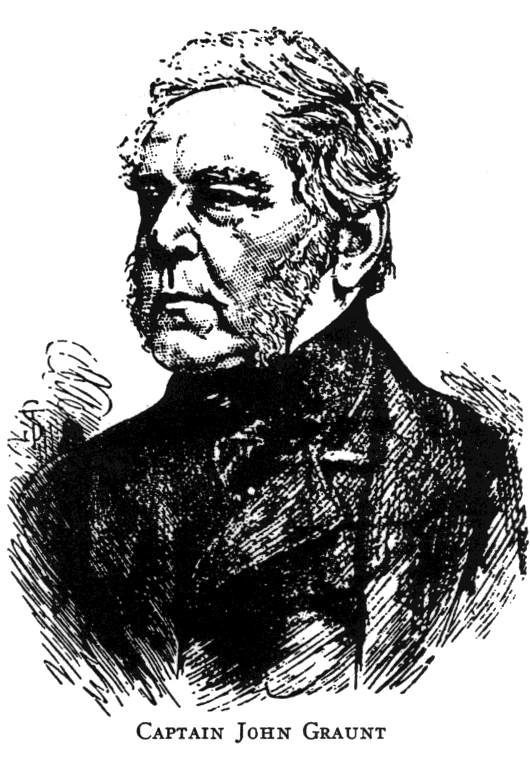
\includegraphics[width=\textwidth]{images/john-graunt.png}
\caption*{\scriptsize
{\bfseries John Graunt} (1620 -- 1674)\\
An early champion of statistics.
}
\end{figure}
\end{minipage}\hspace{0.05\textwidth}%
\begin{minipage}{0.55\textwidth}
\vspace{-2\baselineskip}
Known for early work on:
\vspace{0.5\baselineskip}
\begin{itemize}
    
    \item Descriptive statistics;

    \vspace{0.5\baselineskip}
  
    \item Census methods that lead to modern demography;

    \vspace{0.5\baselineskip}    
    
    \item Epidemiology.

\end{itemize}
\end{minipage}

%https://en.wikipedia.org/wiki/John_Graunt

%Table of Casualties in Natural and Political Observations Made Upon the Bills of Mortality (5th edition, published 1676)

\end{frame}


\section{Where did these techniques come from?}
\begin{frame}{Where did these techniques come from?}


% TODO: Write synopsis and add image:
\begin{minipage}{0.55\textwidth}

\begin{itemize}

\item Fit {\bfseries negative binomial distributions} to the numbers of purchases of a brand of consumer goods.

\vspace{0.5\baselineskip}

\item Modeled repeated category and brand purchases within a wide variety of markets.
% NBD-Dirichlet model of brand choice successfully modelled the

\vspace{0.5\baselineskip}

\item Studied the percentage of the relevant population that has purchased a given brand (or category) at least once in the time period under study.

\end{itemize}

\end{minipage}\hspace{0.05\textwidth}%
\begin{minipage}{0.35\textwidth}
\begin{figure}
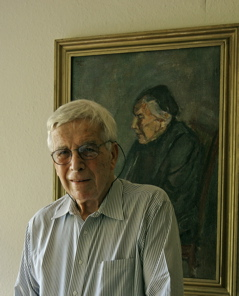
\includegraphics[width=\textwidth]{images/andrew-sc-ehrenberg.jpg}
\caption*{
{\bfseries\scriptsize Andrew S. C. Ehrenberg}\\ Statistician and marketing scientist.
}
\end{figure}
\end{minipage}

\end{frame}

%------------------------------------------%
% A Sprinkle of Economics
%------------------------------------------%
%\section{A Sprinkle of Economics}
%\begin{frame}{A Sprinkle of Economics}
%
%\vspace*{0.125\baselineskip}
%
%\begin{itemize}
%
%\item Cournot
%
%\item Joseph Bertrand
%
%\item Pareto
%
%\item Irving Fisher
%
%\end{itemize}
%
%\end{frame}


%------------------------------------------%
% Application to the Cannabis Industry
%------------------------------------------%
\section{Application to the Cannabis Industry}
\begin{frame}{Application to the Cannabis Industry}

\begin{minipage}{0.45\textwidth}
\begin{center}
\vspace{0.25\baselineskip}
\begin{figure}
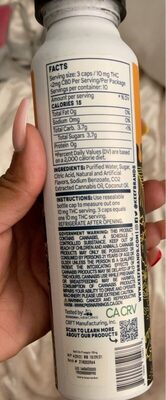
\includegraphics[height=2.5in]{images/beverage-label.jpg}
\vspace{-0.25\baselineskip}
\caption*{
\scriptsize Cannabis--infused beverage label\\[0.125\baselineskip]
\tiny {\color{WildStrawberry} 10mg per serving} | {\color{WildStrawberry} 100mg THC per bottle}\\[0.5\baselineskip]
\tiny\color{Gray}
Author: kiliweb {\tiny https://world.openfoodfacts.org/editor/kiliweb}\\
License: CC BY-SA 3.0 {\tiny https://creativecommons.org/licenses/by-sa/3.0}
}
\end{figure}
\end{center}
\end{minipage}\hspace{0.0\textwidth}%
\begin{minipage}{0.55\textwidth}

\vspace{0.5\baselineskip}

\begin{minipage}{0.75\textwidth}

{\footnotesize\itshape ``Oh Hi’s THC {\color{Mulberry} Pomegranate} Seltzer is our number one seller. When deciding on a new product to launch, we look at \underline{trending flavors}.''}

\vspace{0.5\baselineskip}

{\footnotesize\itshape ``negotiate pricing structures to sell the \underline{customer volume} helps greatly.''}

\vspace{0.5\baselineskip}

{\footnotesize\itshape ``\underline{Expansion can be complex} as it is a capital-intensive investment.''}

\vspace{-0.5\baselineskip}
\begin{flushright}
{\footnotesize - Matt Vincent\\ {\tiny Co-Founder of OH-Hi Beverages}}
\end{flushright}

\end{minipage}

\vspace{0.5\baselineskip}

{\tiny\color{Gray} Reference: https://cannabisdrinksexpo.com/en/blog/producer-profiles-70/consumer-education-is-key-says-matt-vincent-301.htm}

\end{minipage}

% pre-roll brands?

% solid edible brands? Overlap with beverage brands?

% What are the top brands in Washington State and 


\end{frame}


%------------------------------------------%
% Question of the Day
%------------------------------------------%
\section{Question of the Day}
\begin{frame}{Question of the Day}

{\Large {\bfseries Brand Analysis}: Can we measure marketing performance for a cannabis brand?}\\[0.5\baselineskip]

Here is a list of potential metrics:

\vspace{0.25\baselineskip}

\begin{itemize}

\item Market share

\vspace{0.125\baselineskip}

\item Market penetration rate

\vspace{0.125\baselineskip}

\item Purchase frequency / time between purchases

\vspace{0.125\baselineskip}

\item Repeat purchase rate

\vspace{0.125\baselineskip}

\item Items sold

\vspace{0.125\baselineskip}

\item Customer lifetime value

\vspace{0.125\baselineskip}

\item Average product price

\end{itemize}

%\begin{itemize}
%
%\item It is easier to argue that there is natural variance in products such as flower, however, the ability for a beverage manufacturer to capture a large section of the market given a uniform product, typically a 100mg beverage, may depend largely on their marketing effectiveness.
%
%\item Do encumbants get market share?
%
%\item Run the gamut with beverage brand analysis.
%
%\item Using beverage product type for simplicity. The analysis can be readily applied to all product types.
%
%\end{itemize} 

\end{frame}

%------------------------------------------%
% Takeaway
%------------------------------------------%
\section{Takeaway}
\begin{frame}{}

\begin{center}
\begin{minipage}{3.85in}

% Thank you.

\includegraphics[width=.25in]{images/prayer.png} {\Large \textbf{Thank you for coming.}}\\[-0.5\baselineskip]

We've gone over what it means to be a successful {\color{TealBlue} beverage} producer in Washington State and we've seen how data can contain insights for marketers.

\begin{center}
\begin{minipage}{.9\linewidth}
\begin{Block}{Lessons of the Day}

\vspace{0.5\baselineskip}

\begin{itemize}

\item Certain KPIs correlate with {\bfseries market share}:

\vspace{0.25\baselineskip}
\begin{itemize}

\item Market penetration

\vspace{0.25\baselineskip}

\item Product proliferation

\end{itemize}

\vspace{0.25\baselineskip}

\item Spread the word, {\bfseries build your brand}!

\vspace{0.5\baselineskip}

\item {\bfseries Shelf-space}. Get there while you {\itshape can}!

\vspace{0.5\baselineskip}

\end{itemize}

\end{Block}
\end{minipage}
\end{center}

\vfill

\end{minipage}
\end{center}

\vspace{0.5\baselineskip}

What would you like to talk about next week?

\vspace{0.5\baselineskip}

\end{frame}

%------------------------------------------%
% Fin.
%------------------------------------------%
\end{document}
